\subsection{Internal Contrastive Learning (InterCont)}
This chapter examines the internal contrastive learning algorithm proposed by \citet{shenkar2022anomaly}.  The objective is to determine an outlier score $y$, which assigns a low value to samples originating from the underlying distribution, while assigning higher values to potential outliers. 
First I will explain the architecture of the method.
Starting with the construction of the networks and the chosen activation functions.
After that I will proceed with the specific loss function and the normalization that were implemented to estimate the cosine simularity. 
Thereafter I will explain one epoch.
After that I will explain the hyperparameters of the method.
After that I will compare the architecture of the method to the contrastive learning framework explained in the previous section.


The networks architecture comprises two asymmetrical, fully connected neural networks, designated as $F$ and $G$. 
This asymmetry is necessitated by the disparate dimensions of the input vectors $b$ as the anchor and $a$ as the positive sample. 
The authors define the lengths of the hidden layers based on the embedding size $u$.
Network $F$, which processes the larger anchor vector $b$, incorporates two hidden layers: the first containing 200 nodes and the second containing 400 nodes. 
Network $G$ is structured similarly with two hidden layers, yet because it processes the smaller complementary positive sample $a$, the node counts are adjusted accordingly. 
Specifically, the first hidden layer of $G$ consists of 50 nodes, while the second hidden layer consists of 100 nodes. 


The architecture utilizes the LeakyReLU activation function across its layers, with the sole exception of the first hidden layer in Network $F$, which employs a Tanh activation. 
The inclusion of Tanh in the initial layer of the anchor network serves to center the input data and bound activations within the range of -1 to 1, facilitating stability during the early stages of feature extraction for the larger input vector. \todo{review}
LeakyReLU diverges from the standard Rectified Linear Unit by incorporating a small non-zero slope coefficient for negative input values. \todo{previous chapter}
The authors defined this slope coefficient as 0.2. \todo{what does this mean?}
This adjustment prevents the occurrence of dead neurons \todo{different wording} by ensuring that every unit remains capable of contributing to the model's learning process. 
Furthermore, this design ensures that gradients can propagate backward through the network even during negative activations, thereby mitigating the risk of vanishing gradients and allowing for more consistent optimization across the entire network depth.


The authors selected the beforementioned InfoNCE loss function, which serves to maximize the mutual information gain during the training process. \todo{mutual info previous chapter}
This function generates a score that is low for similar data pairs and high for dissimilar pairs. 
Consequently, if a sample does not originate from the underlying distribution, it receives a higher score, indicating a greater probability of being an outlier. \todo{wording}
The specific implementation of the loss function is defined in \ref{INFONCE}


%The numerator of the equation represents the pull between the anchor and the positive sample. \todo{diff place?}
%It is calculated as the product of the anchor and the positive sample, forming the positive pair, which is then divided by the temperature hyperparameter $\tau$. 
%The denominator constitutes the push, represented by the product of the anchor and the negative samples divided by $\tau$. \todo{different wording, push?}
%This product is summed across the total number of negative pairs. 
%Both the numerator and the denominator are processed through a natural exponential function. 
%Consequently, the exponential nature of the scores ensures that higher values exert a disproportionately larger influence on the resulting loss, effectively penalizing the model more severely when the anchor is not sufficiently separated from negative samples or closely aligned with the positive sample.


The authors proposed a sliding window approach for data augmentation to facilitate internal contrastive learning. 
\begin{figure}[htbp]
    \centering
    \begin{minipage}{0.5\textwidth}
        \onehalfspacing
        The model initialization involves treating the columns of the dataset $S$ as a vector $x_i$ with a total length of $d$. 
        The number of pairs $\phi(x_i)={(a_i,b_i)}$ for one instance $x_i$ is determined by the formula $m=d+1-k$, where $k$ represents the defined length of the positive sample $a_i$. 
        The anchor $b_i$ is composed of the residual features $d-k$, functioning as the complementary vector to the positive sample.               
    \end{minipage}
    \hfill 
    \begin{minipage}{0.45\textwidth}
        \centering
        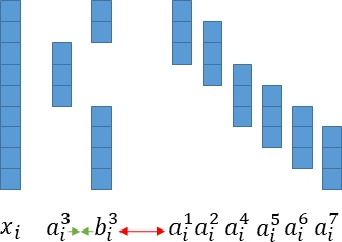
\includegraphics[width=\textwidth]{Images/Shenkar_Wolf}
        \caption{Sliding Window Approach}
    \end{minipage}
    \label{fig:slidinwindow}
\end{figure}


A distinguishing feature of this method is that the negative samples are derived from the positive samples of other constructed pairs within the same data instance, which characterizes the internal nature of the contrastive learning process. 
For a visual representation of this mechanism, see Figure \ref{fig:slidinwindow}


The anchor $b$ will get into the $F$ network and the positive pair $a$ will get into the $G$ network, hence the asymmetrical network structure.
Through the embedding size, the vectors are projected onto a bigger embedding space than before.
Thats a key difference between an autoencoder and this network. 
The network want to learn the comlicated relationsships between the data not the most important features.
The reason is, that tablular often misses internal structre, not like image data.
If a bottleneck architecute were implemented, the networks had do dismiss information to perform the computations, therefore loosing critical information on possible outliers.


The authors implemented different activation function to mitigate the chance that the network simply compare the vectors of similiar datapoints.
The network would have learn class-independend results with no discrimanative power.
So $a$ and $b$ are living in different mathematical spaces.


In the next step, the networks are double normalized and denoted as $F_N$ and $G_N$. 
This process involves two distinct L2-normalization stages for both networks.
This results in unit vectros with different directions.
The initial row-wise normalization is intended to standardize scales across features, as outliers can often be identified simply by the magnitude of a specific feature, resulting in a $L2-Norm$ of 1. 
Thereafter a second column-wise normalization is applied to ensure that each vector is projected onto the surface of a unit hypersphere. 


The the loss function,

\begin{equation}
   \ell(F, G, \Phi(x_i), j) = -\ln \frac{\exp(F^N(b_i^j) \cdot G^N(a_i^j) / \tau)}{\sum_{j'=1}^{m} \exp(F^N(b_i^j) \cdot G^N(a_i^{j'}) / \tau)}
   \label{INFONCE}
\end{equation}


estimates the loss for every pair.
The numerator estimates the simularity of the $b$ and $a$ vector by calculating the dott product.
A higher product indicates a greater degree of similarity between the vectors.


The denominator estimates the simularity between the same $b$ vector but all other $a$ vectors, hence the negative pairs.
By summarizing the dott product of the anchor with all the negative samples and applying it to $exp$ the denominator will always be larger then the numerator and positive.
$-ln$ is implemented to ensure, that the perfect model scores a outlier score of 0 and if the scpore decreases the loss increases.


If $F_N(b_i)*G_N(a_i)=1$ the two vectors point in the identical direction within the feature space.
Conversely, a lower value signifies a lack of similarity, reaching a minimum of -1 when the vectors are diametrically opposed.
Because $G_N(a_i)$ is dissimiliar to $G_N(a_j)$, the cosine simularity of $F_N(b_i)*G_N(a_i)$ should be greater than $F_N(b_i)*G_N(a_j)$, hence the the loss function increases too.
To minimize the loss the euation performs $-ln$ so the result will be small if the result of the term is big. 
The relationsships of the negative pairs are summarized and the loss is calculated.
This procedure is done for all instances.


Through backpropagationg the gradients are estimated and the weights updated.
To mimimize the loss, the methods need to push the negative pairs further appart, decreasing the sum of the dott products in the denominator and holding the dot product of the numinator constant.
The algorithms stops if the loss surpases $10^-3$.  


The sliding window approach has a mayor flaw that it needs dimension with high mutual information lay relatively close to each other.
That is not nececcarly met in tabular data, hence the window is to small to cover those dimensions.
To tackel this, the authors implemented an ensemble learning approach by permutating the dimensions of $S$.
Therefore the methods constructs $r$ number of different versions of $S$. 
And the training will proceed in every version of the table. 
The final loss is estimated by: 

\begin{equation}
    y(x_i) = \frac{1}{r} \sum_{i=1}^{r} y_i(x)
\end{equation}

This ensures that datapoits with a high mutual information will lay in one permutation in the window, resulting in higher robustness and performance.


The model is characterized by three primary hyperparameters:
\begin{enumerate}
    \item $k$ determines the number of consecutive number of the features to form the positive sample $a$.
    \item $u$ determines the embedding size.
    \item $\tau$ is a temperature constant in the contrastive loss function.
\end{enumerate}

If $k$ is set to a big number, the modell could loose its local focus and ignoring important outlier information. 
If $k$ is too small the model cold ignore global relationships and concentrating on local relationships, reducing performance.
For the dataset I used with $d = 127$, the authors determined $k = 2$.


The temperature constant $\tau$ excelerates the differences.
If $\tau$ is small the dott product increases.
In combination with the exponential, small differences between the numerator and the denominator will excelerate.
The authors fixed $\tau = 0.01$.


The embedding size determines how much space the method has to estimate relationsships between the datapoints.
If $u$ is too small, the methods has to discharge information loosing important outlier information. 
If $u$ is too big, it could lead to overfitting.
The authors fixed $u = 200$.


The authors implemented robustness checks.
For $\tau$ and $u$ they could not find volatily in the results.
The best results for my dataset were found with $k=2$.


In comparisog with the fra
To utilize the framework established in the previous sections, the data augmentation techniques specific to InterCont are compared \todo{really comparing?} with conventional contrastive learning strategies. 
Instead of compressing the data, which would be the case in an autoencoder network, the authors chose an expansive architecture. 
The input vectors are projected onto bigger hidden layers.


\todo{add pros and cons}
\todo{insert different papers architecure that apply sliding window approach}
\todo{add: critique}
\todo{define cosine similarity in previous chapter} 